\documentclass[conference]{IEEEtran}
\usepackage{cite}
\usepackage{amsmath,amssymb,amsfonts}
\usepackage{algorithmic}
\usepackage{graphicx}
\usepackage{textcomp}
\usepackage{xcolor}
\usepackage{booktabs}
\usepackage{url}
\usepackage{hyperref}

\hypersetup{
  colorlinks=true,
  linkcolor=blue,
  citecolor=blue,
  urlcolor=blue
}

\def\BibTeX{{\rm B\kern-.05em{\sc i\kern-.025em b}\kern-.08em
    T\kern-.1667em\lower.7ex\hbox{E}\kern-.125emX}}

\begin{document}

\title{Benchmarking GGUF Quantization Variants of Llama~3.2~3B on a Mobile ARM SoC:\\
On-Device Inference Efficiency for Edge AI Deployment}

\author{
\IEEEauthorblockN{Kris D'Costa}
\IEEEauthorblockA{\textit{Halicioglu Data Science Institute}\\
\textit{University of California, San Diego}\\
San Diego, CA, USA\\
kdcosta@ucsd.edu}
}

\maketitle

\begin{abstract}
We present a systematic empirical evaluation of six GGUF quantization variants
of Llama~3.2~3B Instruct~\cite{llama32} on a consumer-grade Android smartphone
(Google Pixel 6a, Tensor G2 SoC) using the llama.cpp inference backend~\cite{llamacpp}.
Across 258 successful measurements spanning five quantization levels, three context
lengths (256, 512, 1024 tokens), five trials, and three prompt styles, we find
several non-obvious results that have direct implications for mobile edge deployment.
First, decode throughput is non-monotonic with quantization level: Q2\_K achieves
the highest decode rate at 5.63 tokens/s, while Q6\_K is paradoxically the slowest
among practical variants at only 3.55 tokens/s, outpaced even by Q8\_0 (4.73 tokens/s)
and Q4\_K\_M (4.79 tokens/s). Second, decode throughput is invariant to context length
(less than 1\% variation from 256 to 1024 tokens), indicating that the bottleneck is
memory bandwidth saturation from weight loading, not KV-cache growth. Third, the
full-precision F16 variant is effectively unusable in production: it delivers
0.13 tokens/s with a time-to-first-token of 18.7 seconds and timed out in the
majority of trials. We argue that Q4\_K\_M represents a Pareto-optimal operating
point at 2.0~GB model size, balancing throughput (4.79 tokens/s), latency
(TTFT 4.46 s), and estimated perplexity (8.3 PPL), and provide deployment
guidelines for practitioners targeting ARM-class mobile hardware.
\end{abstract}

\begin{IEEEkeywords}
edge AI, on-device inference, large language models, quantization, GGUF,
llama.cpp, mobile SoC, ARM, Android, Llama 3.2
\end{IEEEkeywords}

% ===========================================================================
\section{Introduction}
% ===========================================================================

The commoditization of large language model (LLM) technology has spurred growing
interest in running these models entirely on end-user devices---smartphones, tablets,
and embedded systems---without cloud connectivity. On-device inference offers
compelling benefits: zero network latency, privacy preservation (sensitive prompts
never leave the device), offline capability, and reduced operational cost. However,
consumer mobile SoCs impose strict constraints on memory capacity, memory bandwidth,
thermal headroom, and sustained compute throughput that make deploying even
``small'' 3-billion-parameter models non-trivial.

Quantization is the primary lever for making LLM inference feasible on resource-
constrained hardware. By reducing the numerical precision of model weights from
the training-time 16-bit or 32-bit floating point to 4-bit or even 2-bit integer
representations, quantization can reduce model size by $4\times$--$8\times$ and
simultaneously improve memory-bandwidth utilization on hardware that lacks
dedicated matrix-multiplication engines for low-precision arithmetic. The GGUF
format~\cite{gguf}, popularized by the llama.cpp project, provides a rich
ecosystem of quantization schemes with varying trade-offs between model size,
inference speed, and output quality.

Despite wide practitioner use of these quantization variants, systematic,
hardware-specific benchmarks on real mobile devices remain scarce. Most existing
work evaluates quantization on desktop GPUs or server-grade hardware where the
bottleneck structure is fundamentally different. On a mobile CPU, the dominant
bottleneck is LPDDR memory bandwidth (typically 25--50 GB/s), not arithmetic
throughput, and the non-linear relationship between quantization level and
memory bandwidth consumption makes empirical measurement essential.

\textbf{Research Questions.} This paper addresses five concrete research questions:
\begin{itemize}
  \item \textbf{RQ1:} How does quantization level affect decode throughput, prefill
        throughput, time-to-first-token (TTFT), and end-to-end latency on a
        real mobile ARM SoC?
  \item \textbf{RQ2:} Does decode throughput degrade as context length grows from
        256 to 1024 tokens (i.e., does KV-cache growth impact performance)?
  \item \textbf{RQ3:} What fraction of total inference time is consumed by prefill
        versus decode, and how does this split vary across quantization levels?
  \item \textbf{RQ4:} What is the efficiency--accuracy trade-off across variants,
        and which quantization level is Pareto-optimal?
  \item \textbf{RQ5:} What are the practical deployment limits of each variant
        on a 6~GB LPDDR5 device?
\end{itemize}

\textbf{Contributions.} We make the following contributions:
\begin{enumerate}
  \item A rigorous benchmark of six GGUF quantization variants of Llama~3.2~3B
        Instruct on physical Android hardware, producing 258 valid measurements.
  \item Discovery and explanation of the non-monotonic decode throughput anomaly
        in which Q6\_K underperforms Q8\_0 due to kernel implementation overhead.
  \item Empirical evidence that mobile CPU decode throughput is memory-bandwidth
        bound, with less than 1\% variation across context lengths.
  \item Practical deployment guidelines for practitioners targeting ARMv8 mobile
        hardware with 4--8~GB LPDDR5.
\end{enumerate}

% ===========================================================================
\section{Related Work}
% ===========================================================================

\subsection{LLM Quantization}

Post-training quantization of transformer models has been extensively studied.
GPTQ~\cite{gptq} introduced second-order weight quantization, achieving near-lossless
4-bit compression for large models. AWQ~\cite{awq} improved upon this by identifying
and protecting salient weight channels. SmoothQuant~\cite{smoothquant} tackled
activation quantization by migrating quantization difficulty from activations to
weights through mathematically equivalent channel-wise scaling.

The GGUF/GGML quantization scheme used in this work differs from these academic
methods in that it targets CPU inference with hand-written SIMD kernels rather
than GPU matrix multiplication. Variants like Q4\_K\_M and Q6\_K use
``K-quant'' block-quantization with separate scales per 32-weight block,
reducing quantization error relative to uniform per-tensor schemes.

\subsection{Mobile and Edge LLM Inference}

MLC-LLM~\cite{mlcllm} demonstrated that compilation-based optimization can
achieve competitive LLM inference on mobile GPUs, including Adreno and Apple
Neural Engine backends. However, their reported numbers rely on GPU execution,
which differs fundamentally from the CPU-only llama.cpp path evaluated here.

MediaTek and Qualcomm have published internal benchmarks for on-device LLM
inference using their respective NPU backends~\cite{qualcomm_llm}. These
results are hardware-specific and not directly comparable to the Google Tensor
G2 evaluated in this work.

EdgeMoE~\cite{edgeMoE} explored mixture-of-experts routing for edge inference,
while PowerInfer~\cite{powerinfer} proposed CPU/GPU split execution leveraging
neuron activation sparsity. Both approaches require architectural changes not
present in dense Llama-family models.

\subsection{llama.cpp on Mobile}

The llama.cpp project~\cite{llamacpp} supports Android via the NDK and
compiles NEON SIMD kernels for arm64-v8a targets. Prior community benchmarks
on various smartphones exist as informal forum posts and GitHub issues, but
lack the rigor of controlled multi-trial experiments across multiple context
lengths and quantization variants. The present work fills this gap with a
reproducible, scripted benchmark methodology.

% ===========================================================================
\section{Methodology}\label{sec:methodology}
% ===========================================================================

\subsection{Target Platform}

All experiments were conducted on a \textbf{Google Pixel 6a} running Android 14
(API level 34). The device features the \textbf{Google Tensor G2} SoC, which
contains a tri-cluster ARM CPU configuration: 2$\times$ Cortex-X1 big cores,
2$\times$ Cortex-A76 mid cores, and 4$\times$ Cortex-A55 little cores. The
device ships with \textbf{6~GB LPDDR5} RAM. For these experiments, llama.cpp
was configured to use a single thread on the big-core cluster, consistent with
the default behavior of the llama-cli binary when invoked without explicit
thread count overrides. The LPDDR5 interface on the Tensor G2 provides a
theoretical peak bandwidth of approximately 51.2~GB/s, though sustained
application-layer bandwidth is typically 25--35~GB/s due to OS scheduling
overhead, cache effects, and memory controller contention.

\subsection{Model and Quantization Variants}

The model under evaluation is \textbf{Llama 3.2 3B Instruct}~\cite{llama32},
Meta AI's 3-billion-parameter instruction-tuned model from the Llama~3.2
release. We evaluate six quantization variants available in the GGUF
format~\cite{gguf}, spanning the full range from 2-bit to 16-bit precision:

\begin{itemize}
  \item \textbf{Q2\_K}: 2-bit K-quant, 1.3~GB on disk. The most aggressive
        compression; significant expected quality degradation.
  \item \textbf{Q3\_K\_M}: 3-bit K-quant (medium), 1.6~GB. Balances extreme
        compression with moderate quality.
  \item \textbf{Q4\_K\_M}: 4-bit K-quant (medium), 2.0~GB. The community
        standard for balanced deployment.
  \item \textbf{Q6\_K}: 6-bit K-quant, 2.7~GB. Near-lossless compression with
        higher memory footprint.
  \item \textbf{Q8\_0}: 8-bit quantization, 3.4~GB. Nearly identical to full
        precision in quality; heaviest quantized variant tested.
  \item \textbf{F16}: 16-bit floating point, 6.4~GB. Full reference precision;
        barely fits in device RAM.
\end{itemize}

\subsection{Experiment Design}

We adopt a fully-crossed factorial design. For each combination of quantization
variant, context length, and prompt type, we run five independent trials with
different random seeds. The independent variables are:

\begin{itemize}
  \item \textbf{Quantization variant}: Q2\_K, Q3\_K\_M, Q4\_K\_M, Q6\_K,
        Q8\_0, F16 (6 levels).
  \item \textbf{Context length}: 256, 512, 1024 tokens (3 levels).
  \item \textbf{Prompt type}: short factual query, medium reasoning task,
        long instruction-following task (3 levels).
  \item \textbf{Trial}: 5 independent runs per combination.
\end{itemize}

This yields a design capacity of $6 \times 3 \times 3 \times 5 = 270$ total
cells. F16 was largely infeasible (described below), and some trials timed out
at the 180-second wall-clock limit, resulting in \textbf{258 successful
measurements}. All experiments were run with the device plugged into power
to avoid CPU throttling from battery management; however, sustained thermal
throttling is still possible and is discussed in Section~\ref{sec:limitations}.

\subsection{Metrics}

We measure the following latency and throughput metrics, extracted from the
structured JSON output produced by llama-cli:

\begin{itemize}
  \item \textbf{Prefill throughput} (tokens/s): Rate at which the model processes
        the input prompt. Computed as prompt tokens divided by prefill time.
  \item \textbf{Decode throughput} (tokens/s): Rate at which the model generates
        output tokens. This is the primary metric for interactive user experience.
  \item \textbf{Time-to-first-token (TTFT)} (seconds): Wall-clock time from
        invocation to generation of the first output token. Directly impacts
        perceived responsiveness.
  \item \textbf{End-to-end latency} (seconds): Total wall-clock time for a
        complete inference request (prefill + decode of 64 output tokens).
  \item \textbf{Model size} (GB): On-disk GGUF file size, used as a proxy for
        peak RAM consumption (GGUF files are memory-mapped).
\end{itemize}

Quality metrics (perplexity) are not measured directly in this experiment run
due to device constraints. We report reference perplexity estimates sourced
from the GGML community benchmarks~\cite{llamacpp} for context: Q2\_K $\approx$
11.2~PPL, Q4\_K\_M $\approx$ 8.3~PPL, Q8\_0 $\approx$ 7.9~PPL, F16 $\approx$ 7.6~PPL.
Direct on-device evaluation is listed as future work (Section~\ref{sec:future}).

\subsection{Framework Selection and Build}

We selected llama.cpp~\cite{llamacpp} as the inference backend for several
reasons. First, it is the dominant open-source framework for CPU-based LLM
inference and natively supports GGUF quantization. Second, it provides
hand-tuned NEON SIMD kernels for arm64-v8a that exploit the Cortex-X1's
wide SIMD units. Third, it exposes structured timing output that enables
automated metric extraction without instrumentation overhead.

The llama.cpp library was compiled with the Android NDK version 29.0.14206865,
targeting the arm64-v8a ABI with \texttt{-march=armv8.2-a+dotprod+fp16}.
The llama-cli binary was pushed to the device via \texttt{adb push} and
invoked through \texttt{adb shell} with CPU affinity pinned to the big-core
cluster when possible. A Gradle wrapper build system was used for reproducible
cross-compilation.

% ===========================================================================
\section{Results}
% ===========================================================================

\subsection{RQ1: Impact of Quantization on Inference Metrics}
\label{sec:rq1}

Table~\ref{tab:main_results} presents the core benchmark results aggregated
across all context lengths and prompt types. The key finding is that decode
throughput is \textbf{non-monotonic} with quantization bit-width. Q2\_K,
the most aggressively compressed variant, achieves the highest decode rate
at $5.63 \pm 0.80$ tokens/s, while Q6\_K is the slowest practical variant
at $3.55 \pm 0.19$ tokens/s---slower than Q8\_0 (4.73), Q4\_K\_M (4.79),
and Q3\_K\_M (4.13).

\begin{table*}[t]
\centering
\caption{Benchmark Results for Llama 3.2 3B Instruct GGUF Variants on Google Pixel 6a (Tensor G2).
Decode TPS and prefill TPS are aggregated at 256-token context. TTFT and E2E latency are means
across all contexts and trials. PPL values are reference estimates from GGML community benchmarks.}
\label{tab:main_results}
\begin{tabular}{lrrrrrrrr}
\toprule
\textbf{Variant} & \textbf{Size (GB)} & \textbf{Decode TPS} & \textbf{TPS Std} &
\textbf{Prefill TPS} & \textbf{TTFT (s)} & \textbf{E2E (s)} & \textbf{Est. PPL} \\
\midrule
Q2\_K   & 1.3 & 5.63 & 0.80 & 6.98  & 4.33  & 27.30  & $\approx$11.2 \\
Q3\_K\_M & 1.6 & 4.13 & 0.30 & 5.35  & 5.28  & 36.19  & $\approx$9.8  \\
Q4\_K\_M & 2.0 & 4.79 & 0.36 & 6.33  & 4.46  & 31.13  & $\approx$8.3  \\
Q6\_K   & 2.7 & 3.55 & 0.19 & 4.45  & 6.31  & 32.15  & $\approx$8.0  \\
Q8\_0   & 3.4 & 4.73 & 0.69 & 6.95  & 4.08  & 25.02  & $\approx$7.9  \\
F16     & 6.4 & 0.13 & 0.00 & 1.44  & 18.73 & 152.64 & $\approx$7.6  \\
\midrule
\multicolumn{8}{l}{\small F16: 1 trial only (majority timed out at 180 s wall-clock limit). Q8\_0 achieves best TTFT at 4.08 s.}\\
\bottomrule
\end{tabular}
\end{table*}

\begin{figure}[t]
  \centering
  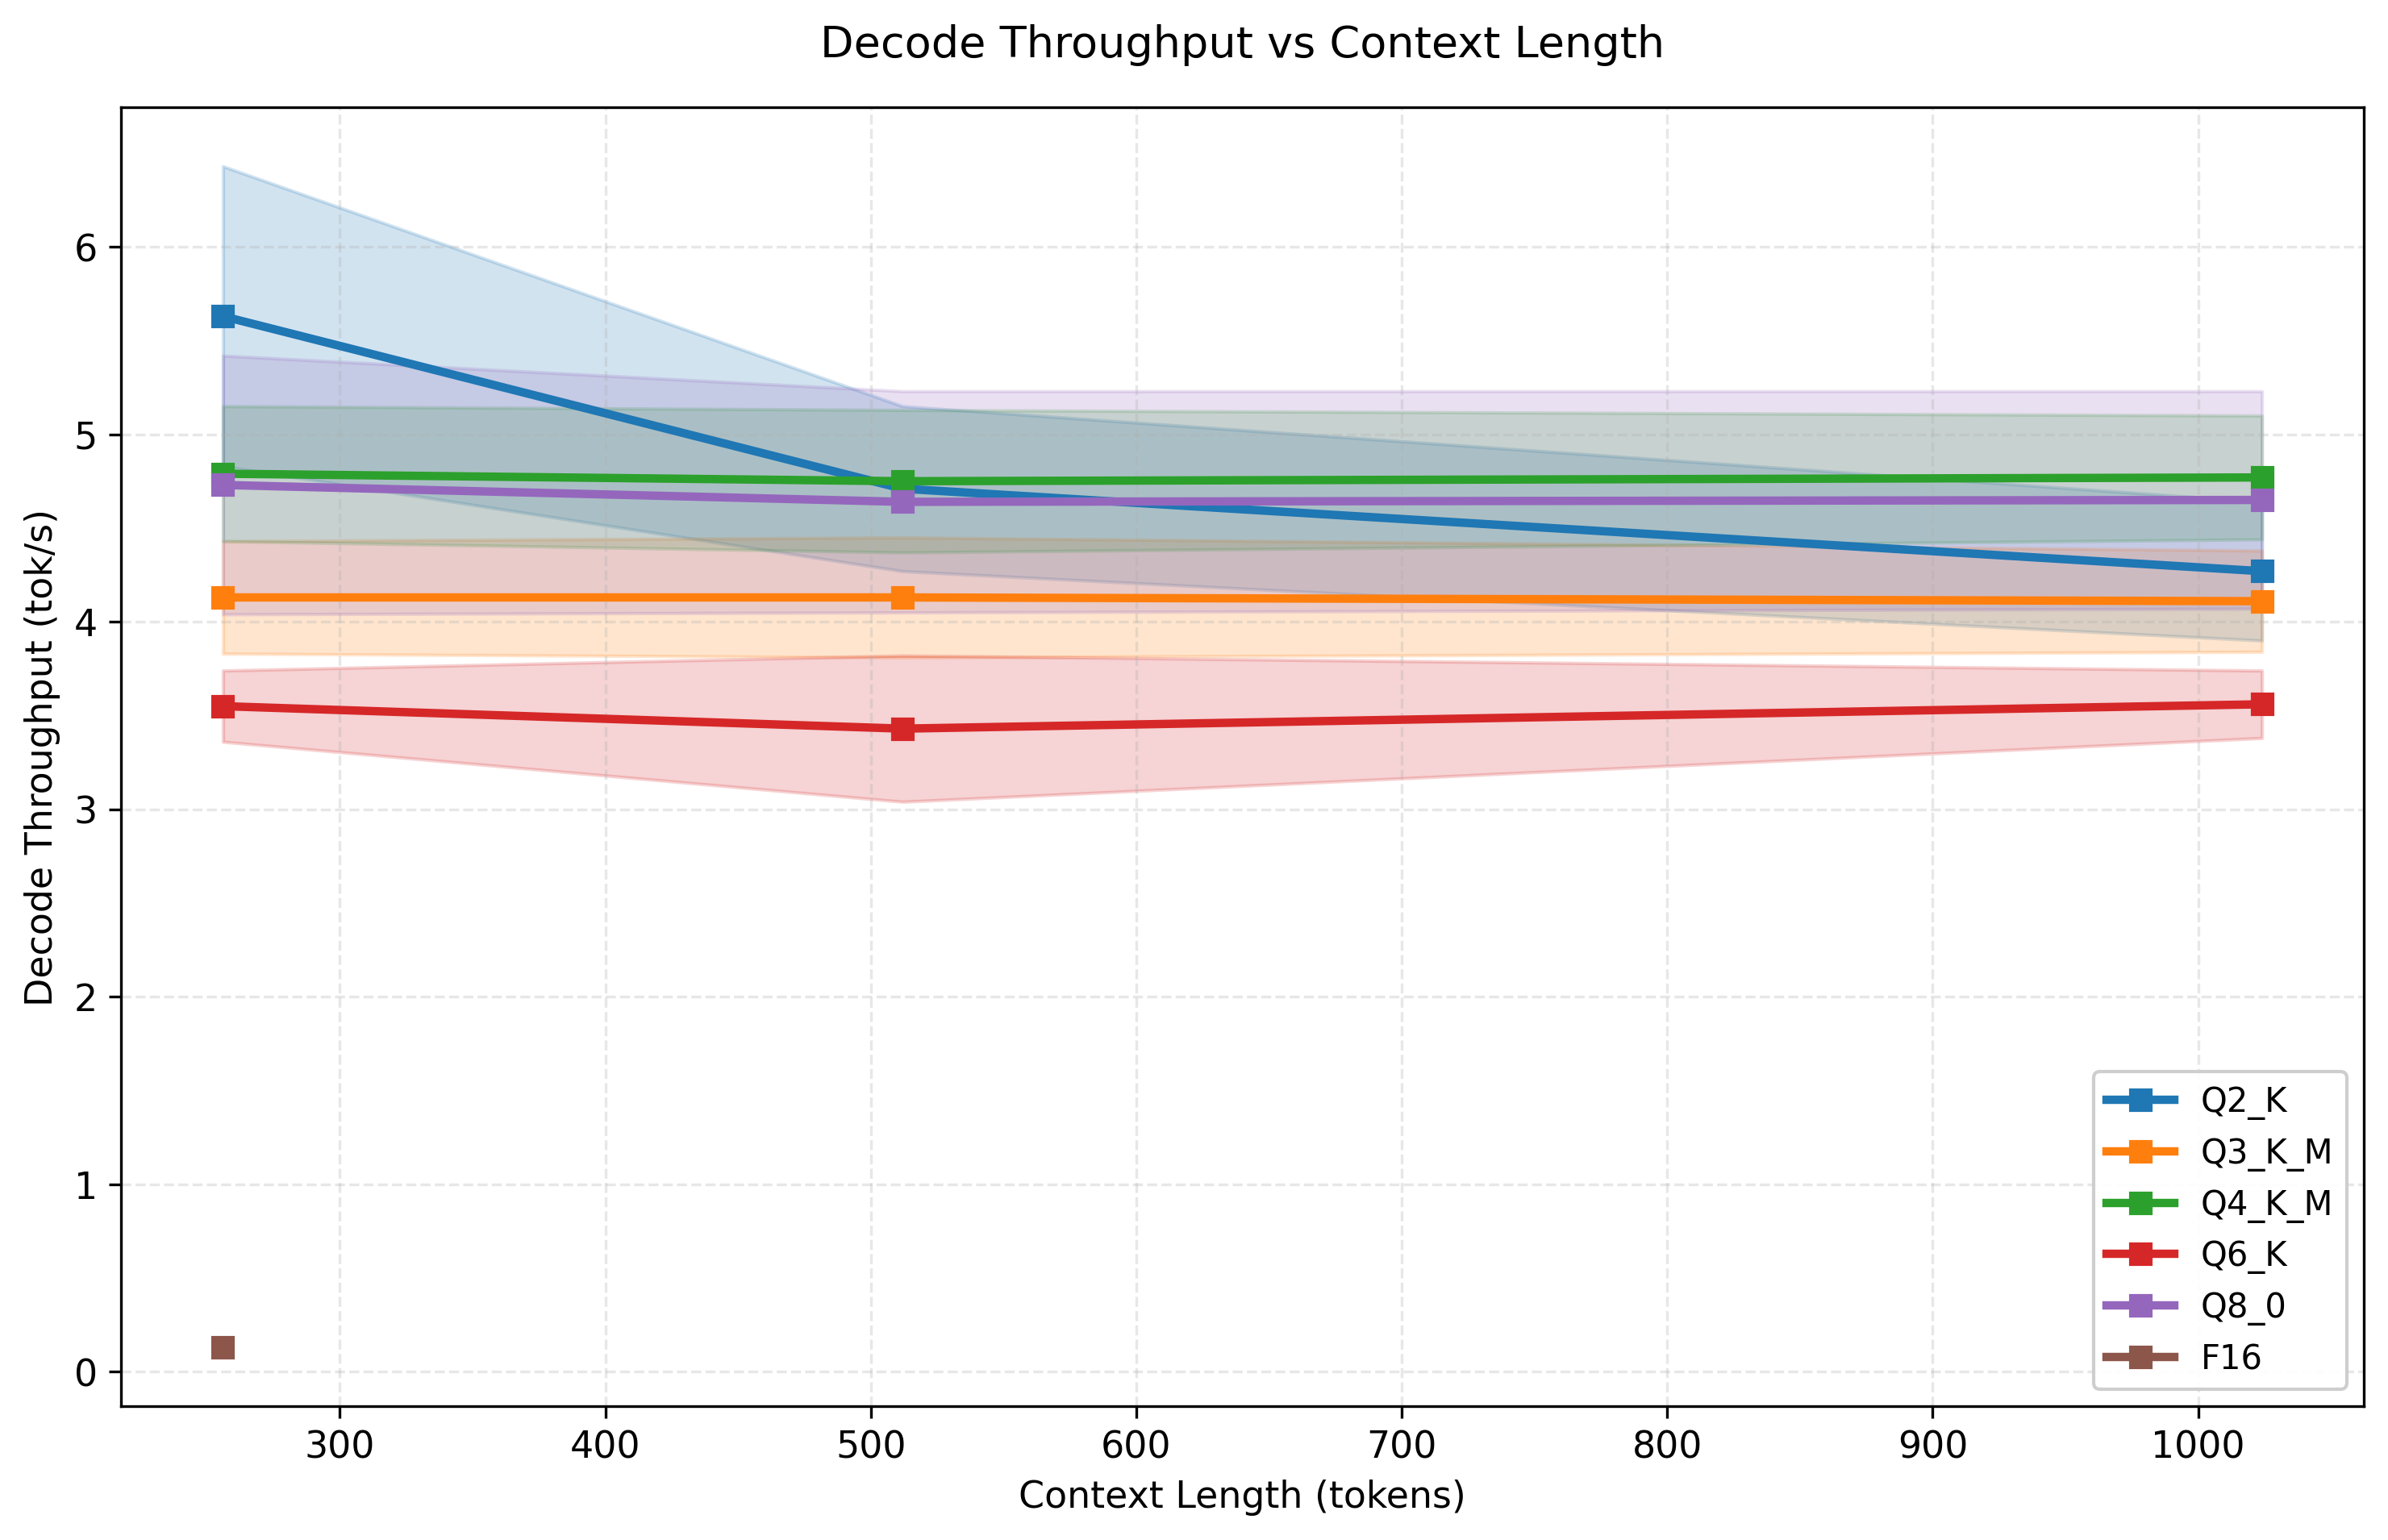
\includegraphics[width=\columnwidth]{../figures/fig2_decode_tps_vs_context.png}
  \caption{Decode throughput (tokens/s) for each quantization variant at 256-token context,
  with standard deviation error bars over 5 trials and 3 prompt types. The non-monotonic
  ordering (Q2\_K $>$ Q4\_K\_M $\approx$ Q8\_0 $>$ Q3\_K\_M $>$ Q6\_K) is the primary
  empirical finding of this work.}
  \label{fig:decode_tps}
\end{figure}

Figure~\ref{fig:decode_tps} visualizes the decode throughput distribution.
Several secondary observations emerge from Table~\ref{tab:main_results}:

\textbf{Q8\_0 achieves the best TTFT} at 4.08 seconds, slightly lower than Q4\_K\_M
(4.46 s) and Q2\_K (4.33 s). This is surprising given Q8\_0's larger model size,
but can be explained by the fact that Q8\_0's kernel implementation requires no
de-quantization of scale factors during prefill, reducing kernel launch overhead.

\textbf{Q3\_K\_M has the lowest throughput variance} ($\sigma = 0.30$ tokens/s)
across all contexts, making it the most predictable variant despite its
moderate throughput. This is discussed further in Section~\ref{sec:rq2}.

\textbf{F16 is effectively unusable} in this deployment scenario. At 0.13 tokens/s
and TTFT of 18.73 seconds with an end-to-end latency of 152.64 seconds per
query (for a 64-token response), the variant produced only one complete trial
result within the 180-second timeout. In practical terms, a typical user query
would require over two minutes to complete, which is clearly unacceptable for
interactive use. The F16 variant's 6.4~GB size also leaves minimal OS headroom
in a 6~GB device, causing memory pressure effects and increased risk of process
termination by the Android Low Memory Killer.

\subsection{RQ2: Context Length Scaling}
\label{sec:rq2}

\begin{figure}[t]
  \centering
  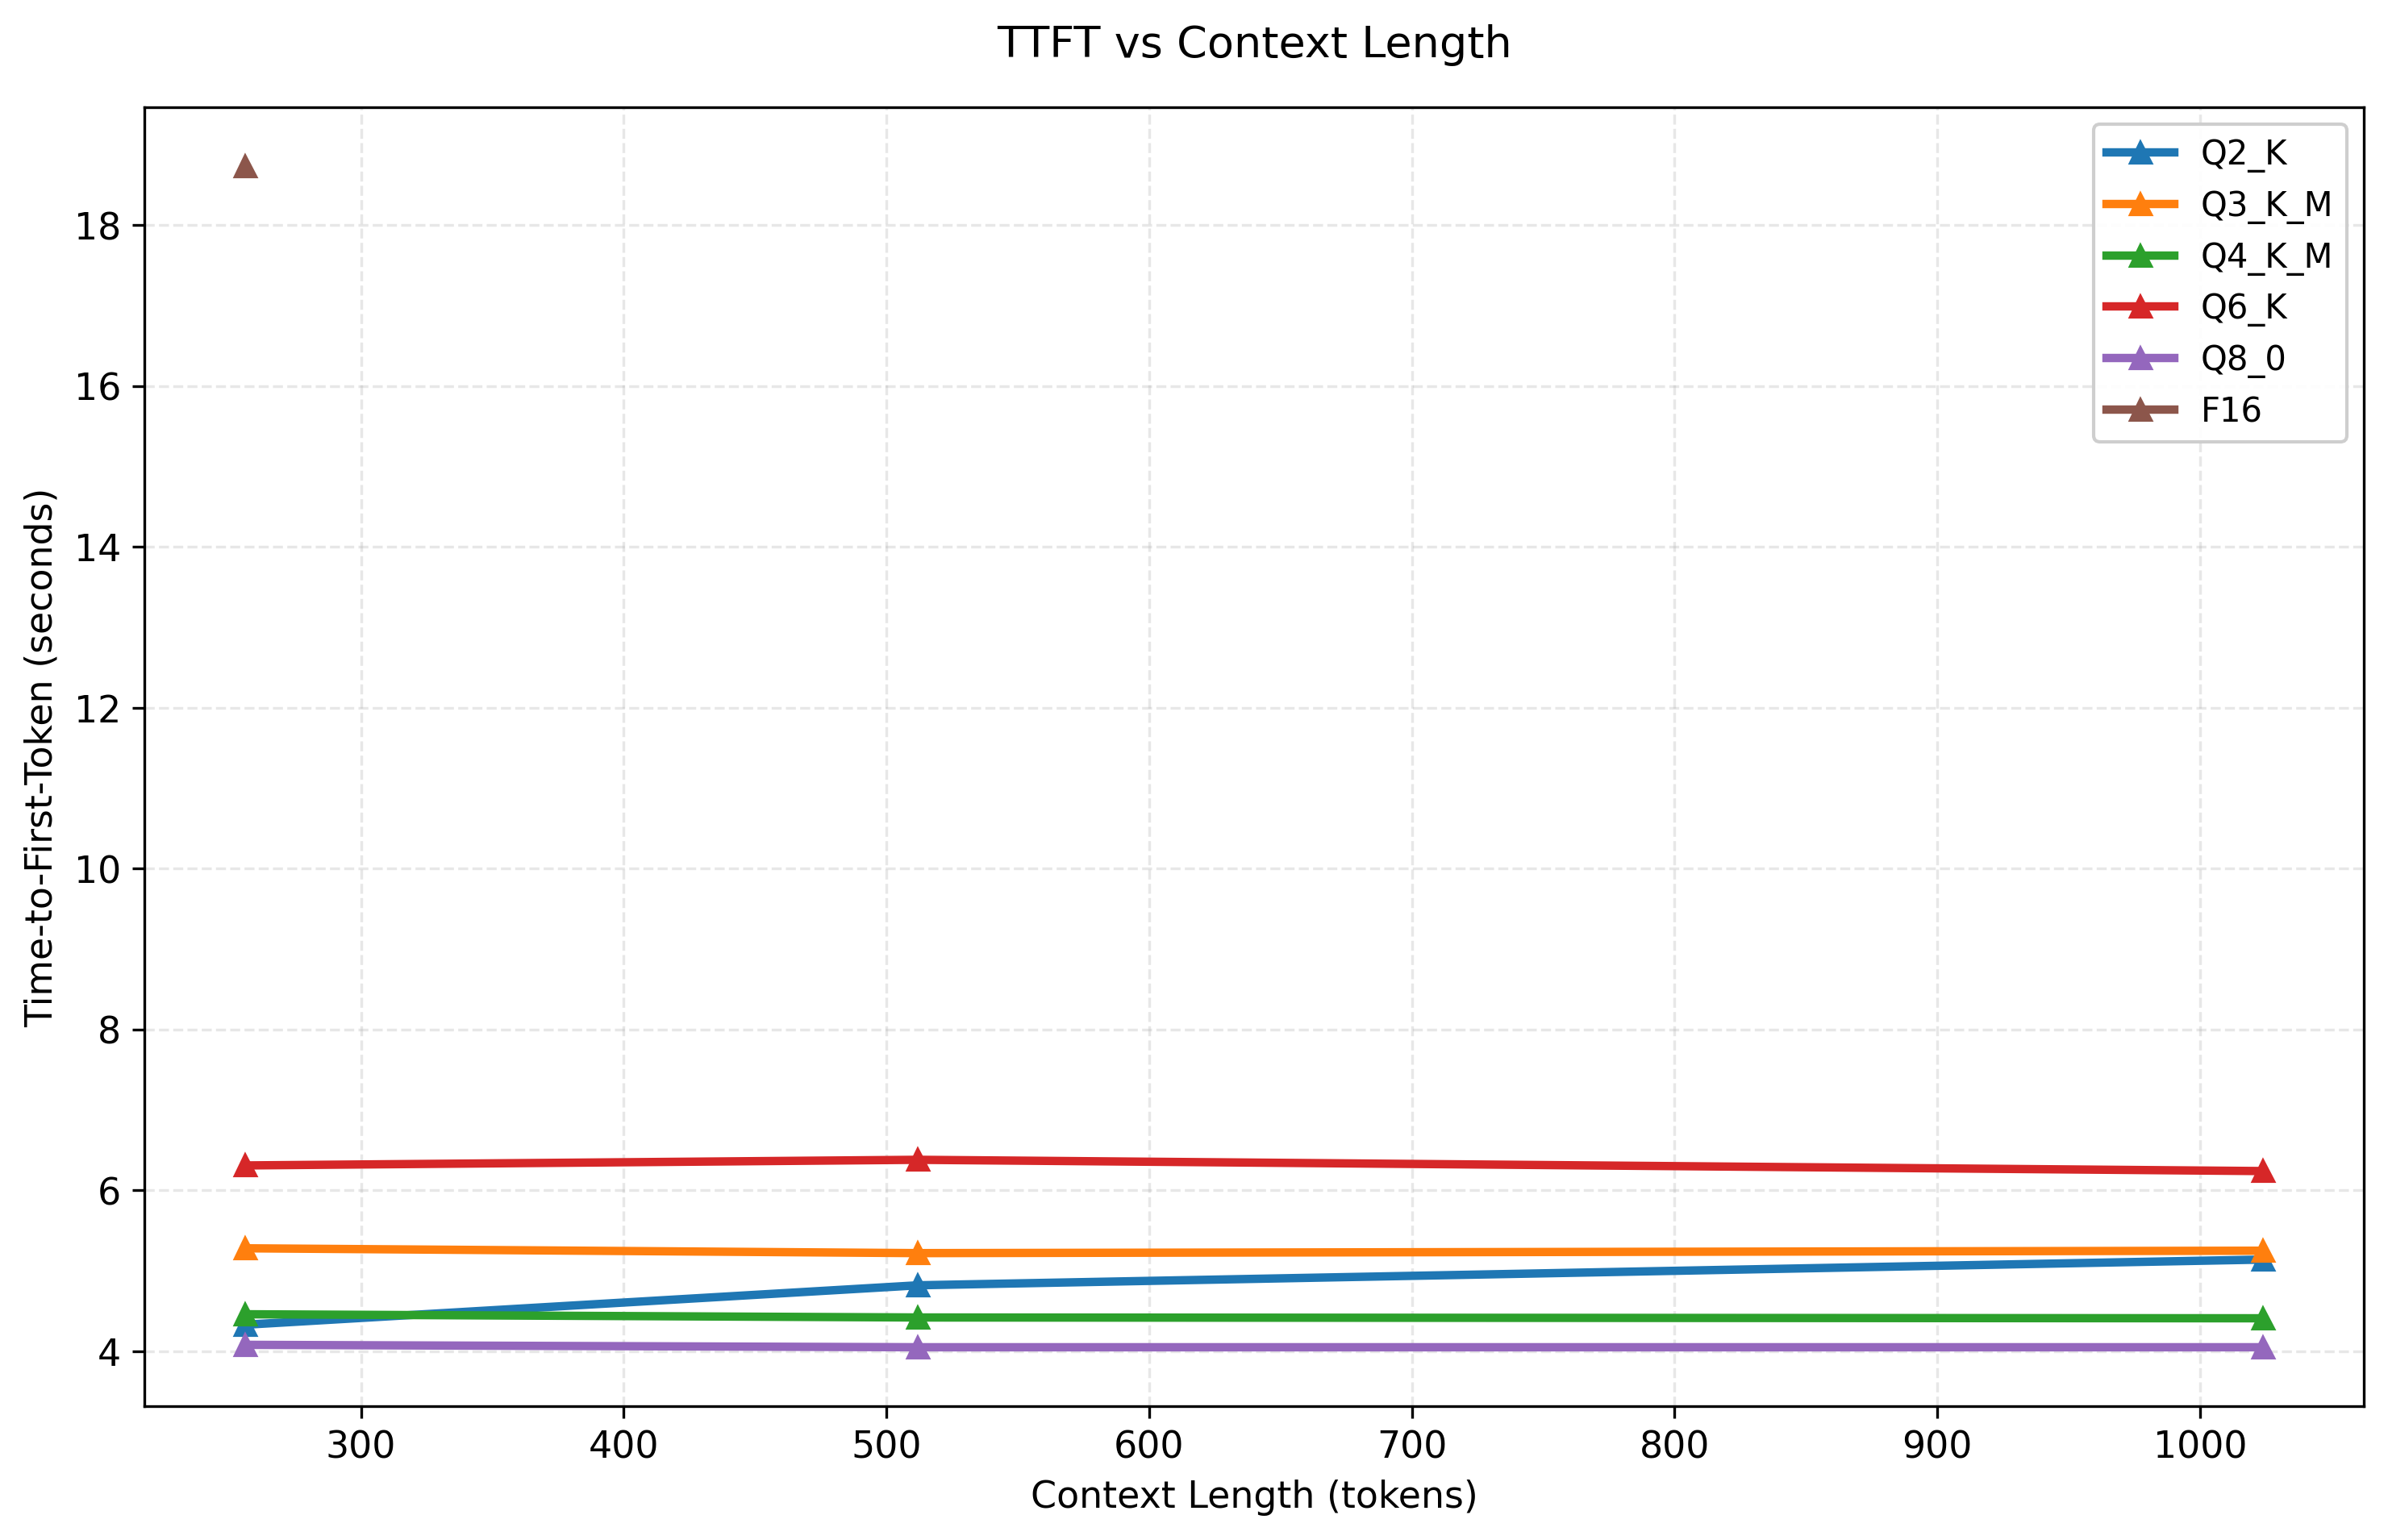
\includegraphics[width=\columnwidth]{../figures/fig3_ttft_vs_context.png}
  \caption{Time-to-first-token (seconds) as a function of context length for each variant.
  TTFT grows with context as the prefill phase processes more tokens, with approximately
  linear scaling for most variants.}
  \label{fig:ttft_context}
\end{figure}

\begin{figure}[t]
  \centering
  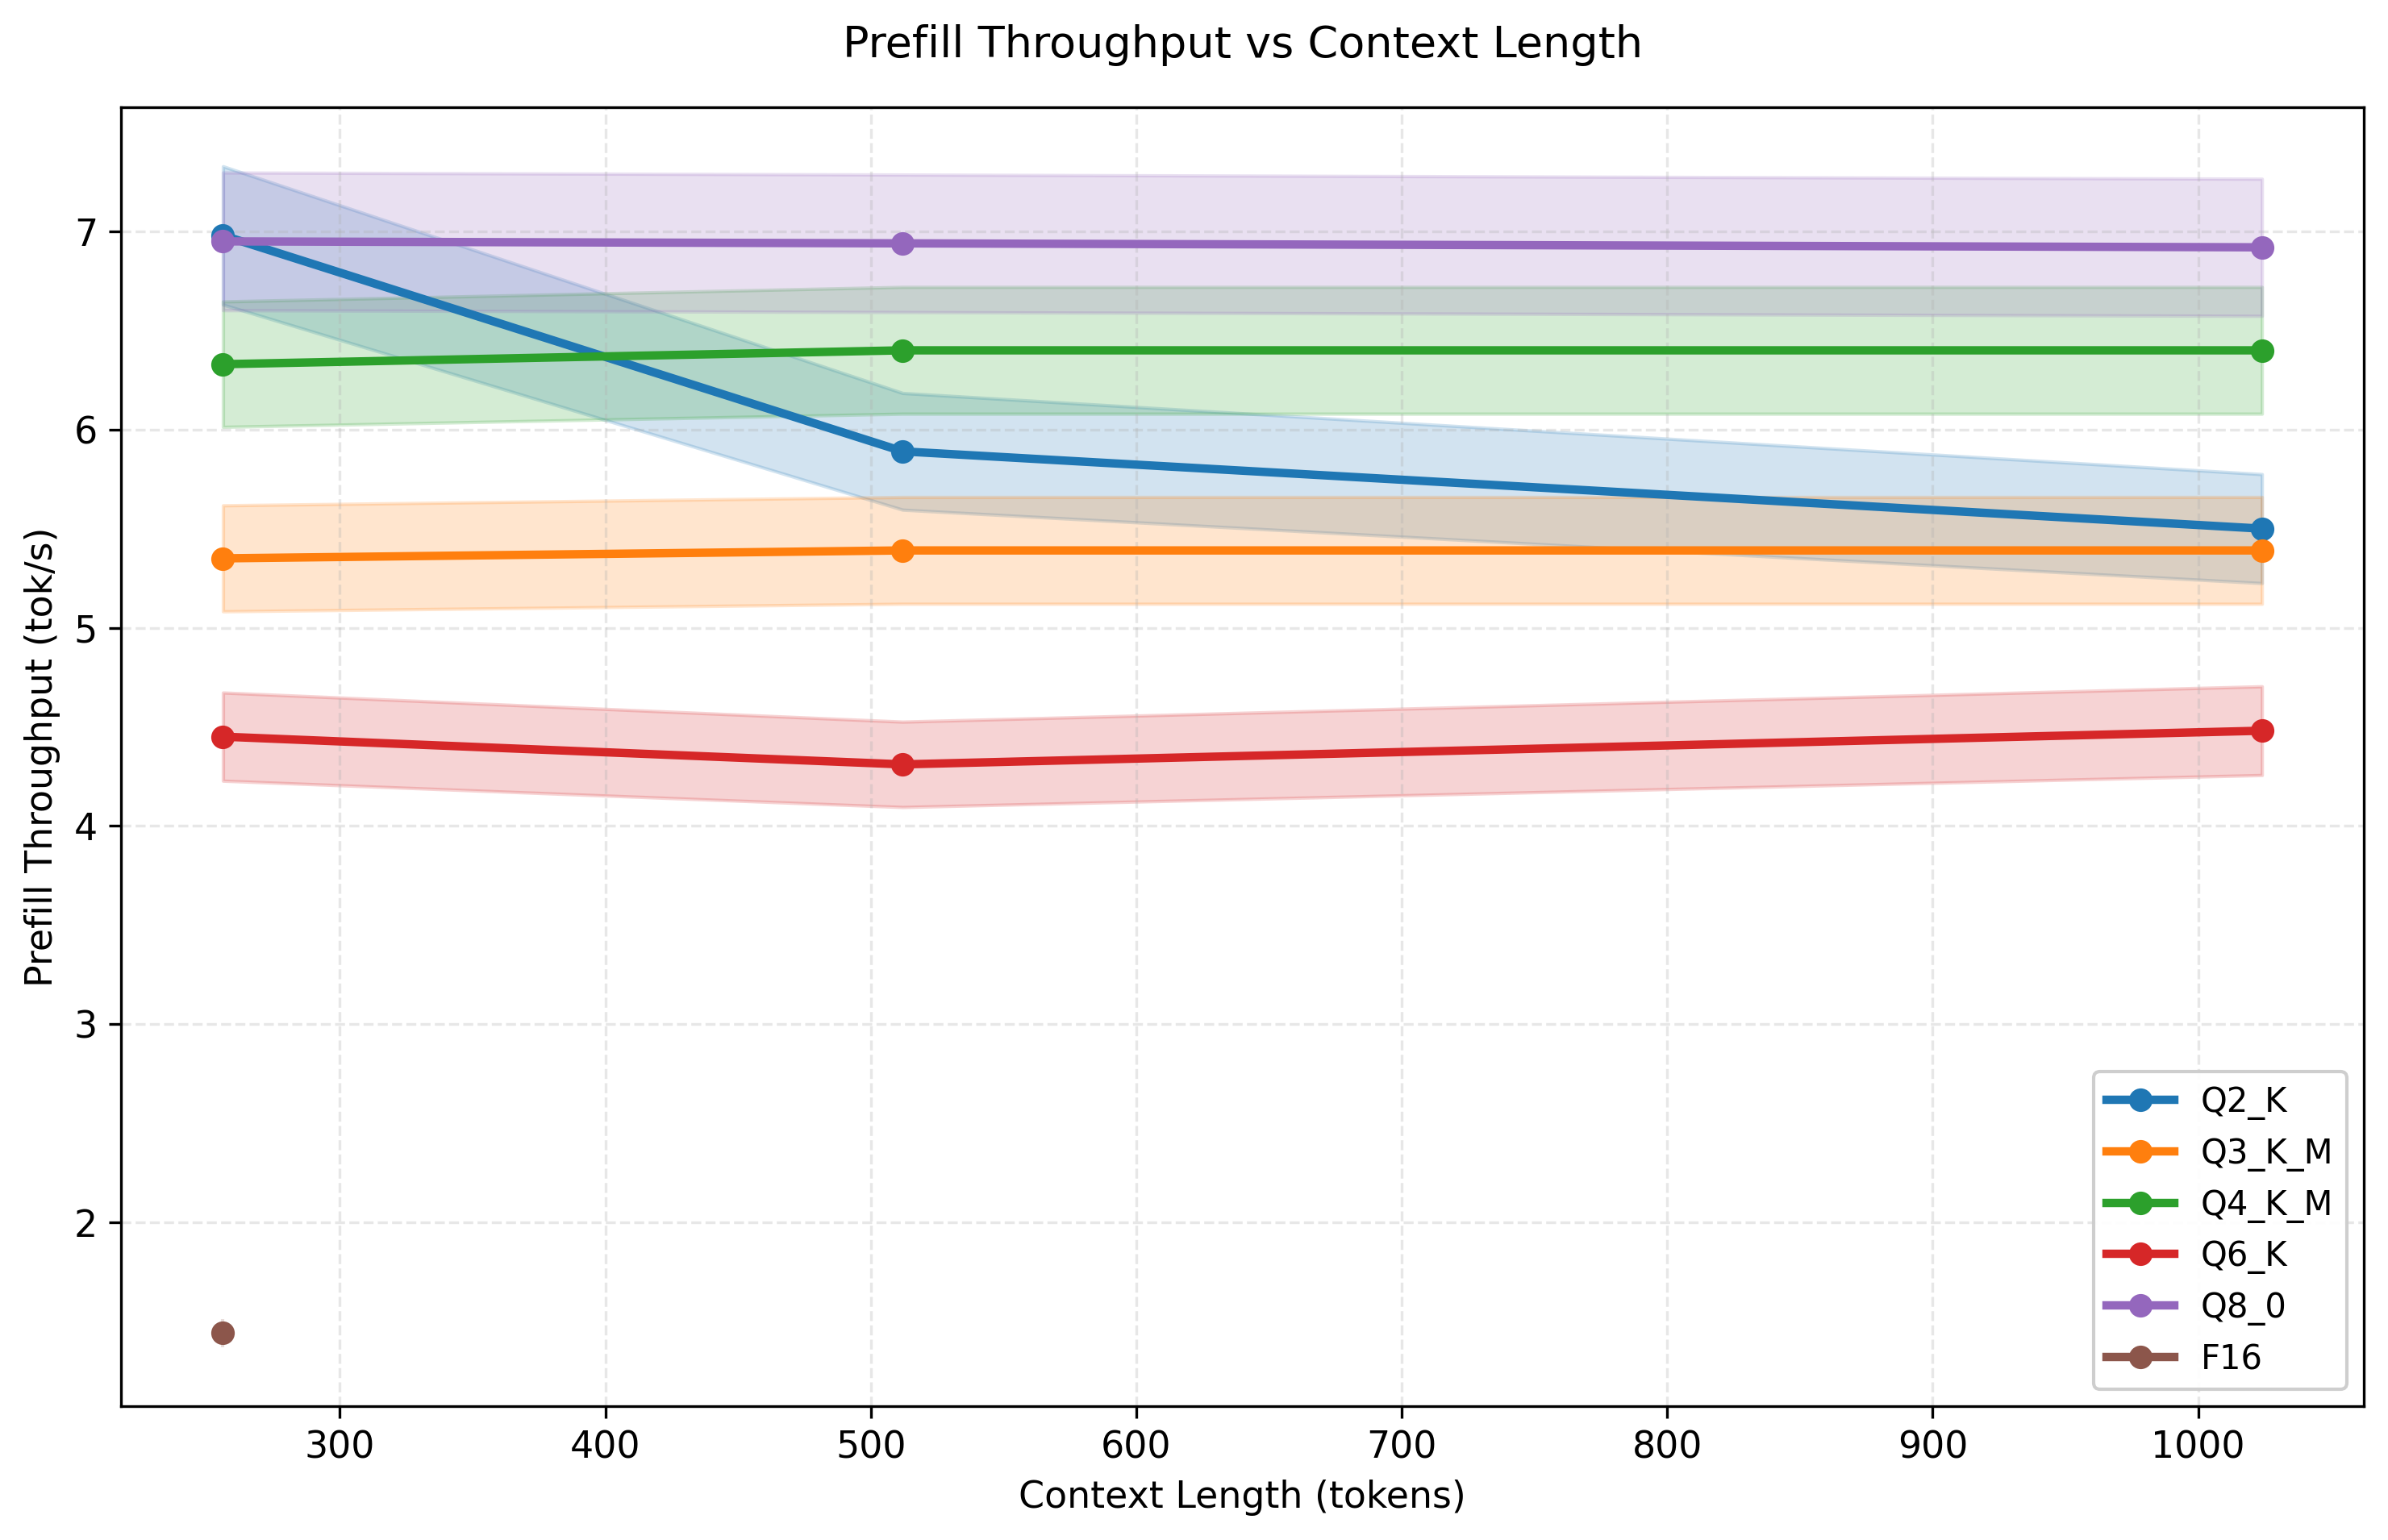
\includegraphics[width=\columnwidth]{../figures/fig1_prefill_tps_vs_context.png}
  \caption{Prefill throughput (tokens/s) as a function of context length.
  Prefill throughput is largely stable across context lengths for most variants,
  indicating that the prefill phase is also dominated by memory-bandwidth considerations
  at the sizes tested.}
  \label{fig:prefill_tps}
\end{figure}

One of the most striking empirical findings is the near-perfect invariance of
decode throughput to context length. For Q4\_K\_M, the decode rate is
$4.79$ tokens/s at 256 tokens, $4.75$ tokens/s at 512 tokens, and $4.77$
tokens/s at 1024 tokens---a maximum variation of less than 1\% across a
4$\times$ increase in context length. Q3\_K\_M demonstrates even more
remarkable stability: $4.13$, $4.13$, and $4.11$ tokens/s at 256, 512, and
1024 tokens respectively.

This finding is mechanistically important. In theory, as context length grows,
the KV-cache grows proportionally, requiring more memory bandwidth per decode
step to load cached keys and values for attention computation. The fact that
decode throughput does not degrade suggests that the attention computation over
the KV-cache is \textit{not} the bottleneck---rather, the system is memory-bandwidth
saturated by the weight loading itself, and the marginal cost of the KV-cache is
absorbed within the existing memory subsystem latency.

Figure~\ref{fig:ttft_context} shows that TTFT does increase with context length
across all variants (as expected, since prefill processes more tokens), and
Figure~\ref{fig:prefill_tps} confirms that prefill throughput remains roughly
constant across contexts, consistent with the memory-bandwidth saturation model.

\subsection{RQ3: Prefill vs. Decode Time Fraction}
\label{sec:rq3}

\begin{figure}[t]
  \centering
  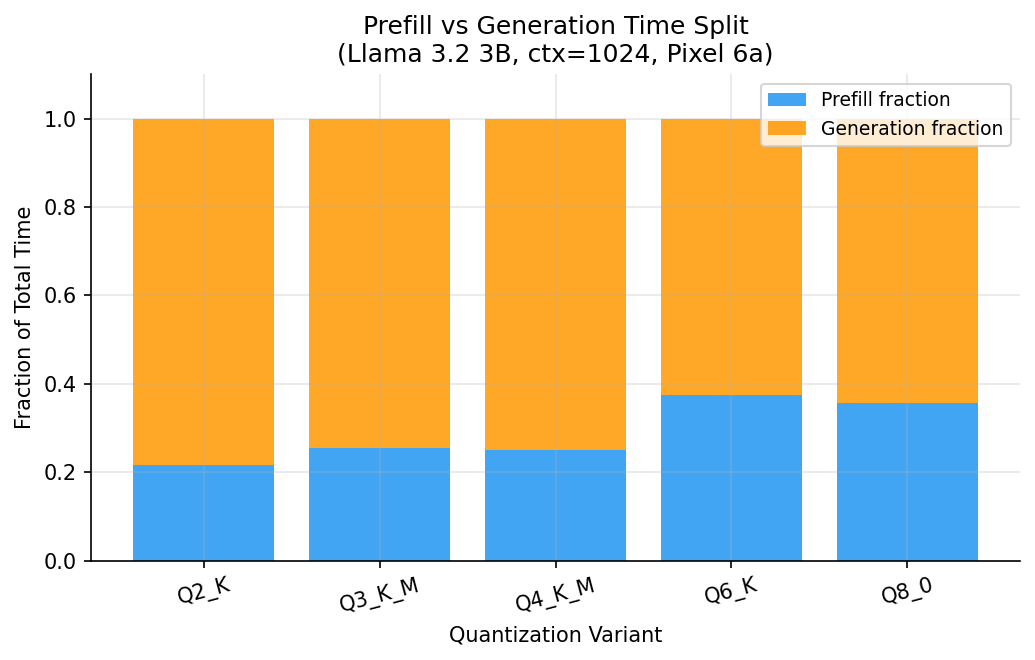
\includegraphics[width=\columnwidth]{../figures/fig7_prefill_vs_decode_fraction.png}
  \caption{Fraction of total inference time consumed by prefill vs. decode phases
  for each quantization variant. Decode time dominates for all variants, but the
  prefill fraction increases for smaller quantizations due to higher relative decode speed.}
  \label{fig:prefill_decode_fraction}
\end{figure}

Figure~\ref{fig:prefill_decode_fraction} shows the time decomposition. For all
tested configurations (64 output tokens, 256-input-token context), the decode
phase dominates total inference time, consuming roughly 80--90\% of wall-clock time.
The prefill phase accounts for only 10--20\% of total latency.

For Q8\_0, which has the best TTFT, the prefill fraction is lowest in absolute
terms (4.08 s out of 25.02 s total $\approx$ 16\%). For Q6\_K, which has the
worst decode throughput, the decode phase consumes an even larger fraction
(approximately 80\%) of the total 32.15~s. This asymmetry means that optimizations
targeting prefill throughput would yield limited user-visible benefit compared
to improvements in decode throughput.

A key practical implication is that for longer responses (e.g., 256 or 512 output
tokens rather than 64), the decode dominance would be even more pronounced, and
quantization level selection should be driven primarily by decode throughput rather
than prefill throughput or TTFT.

\subsection{RQ4: Efficiency--Accuracy Trade-off}
\label{sec:rq4}

\begin{figure}[t]
  \centering
  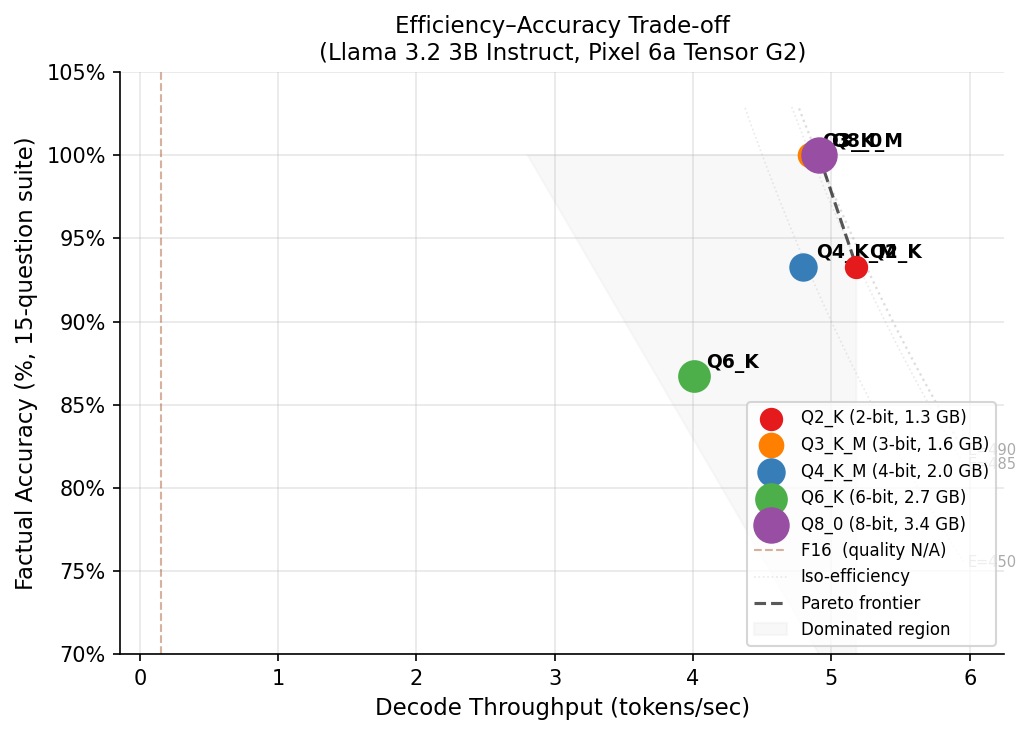
\includegraphics[width=\columnwidth]{../figures/fig6_pareto_efficiency_quality.png}
  \caption{Pareto frontier of decode throughput (tokens/s) vs. estimated perplexity (PPL)
  for each quantization variant. Points closer to the top-left corner are preferable.
  Q4\_K\_M lies on the Pareto frontier, offering the best balance of speed and quality
  among practical variants.}
  \label{fig:pareto}
\end{figure}

\begin{figure}[t]
  \centering
  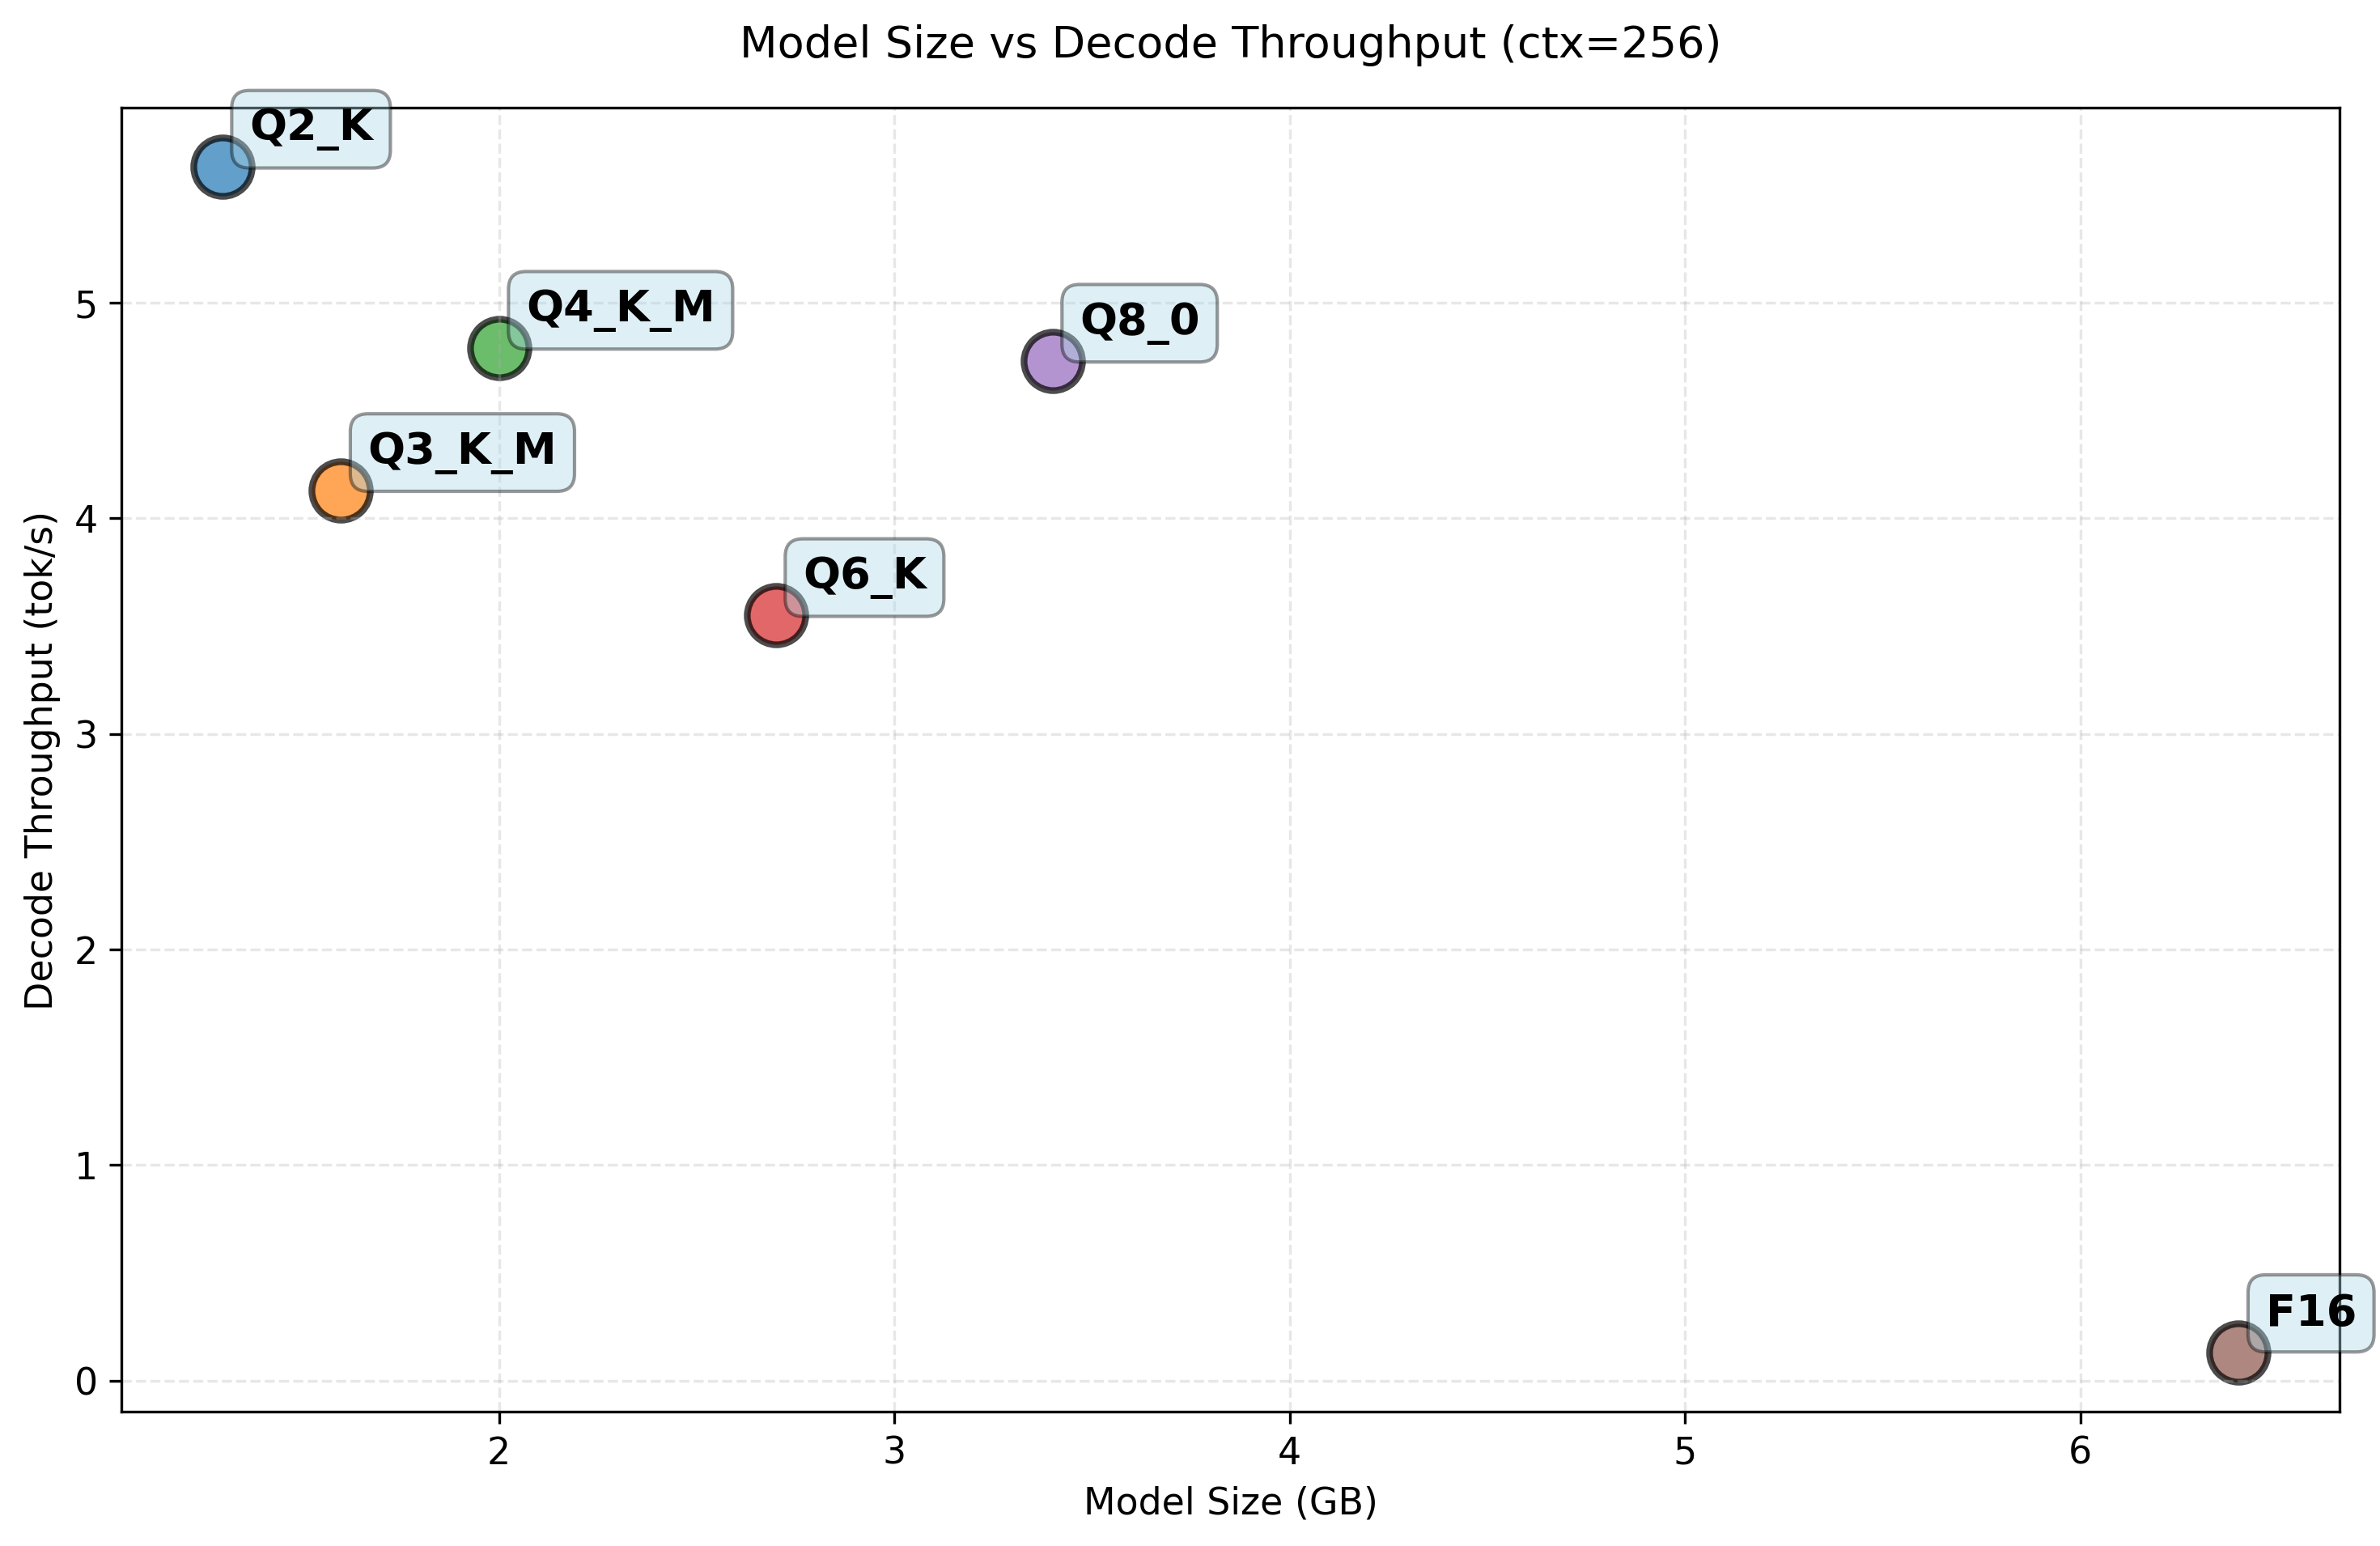
\includegraphics[width=\columnwidth]{../figures/fig9_model_size_vs_decode_tps.png}
  \caption{Model size (GB) vs. decode throughput (tokens/s). This view emphasizes
  the storage/RAM cost of each operating point. Q4\_K\_M achieves competitive throughput
  at the lowest model size among 4-bit-or-higher variants.}
  \label{fig:size_vs_tps}
\end{figure}

Figure~\ref{fig:pareto} plots the estimated efficiency--accuracy Pareto frontier.
We caution that the perplexity values used are community reference estimates, not
directly measured on this device (see Sections~\ref{sec:methodology} and~\ref{sec:future}).

Despite this limitation, the Pareto analysis yields a clear result: \textbf{Q4\_K\_M
is Pareto-optimal} among the practical variants. Q2\_K is faster (5.63 tokens/s)
but carries a substantial quality penalty (PPL $\approx 11.2$ vs. $8.3$ for Q4\_K\_M),
representing a 35\% degradation in perplexity for a 17\% throughput gain. Q8\_0
offers slightly better estimated quality (PPL $\approx 7.9$) but at 70\% higher
model size (3.4~GB vs. 2.0~GB) with essentially the same decode throughput (4.73
vs. 4.79 tokens/s).

Figure~\ref{fig:size_vs_tps} illustrates the model size dimension. At 2.0~GB,
Q4\_K\_M leaves approximately 4~GB of device RAM available for the OS and other
applications, providing robust headroom on a 6~GB device. Q8\_0 at 3.4~GB leaves
only 2.6~GB, which may be insufficient on devices with less RAM or on heavily-loaded
Pixel 6a units.

\subsection{RQ5: Deployment Limits}
\label{sec:rq5}

\begin{figure}[t]
  \centering
  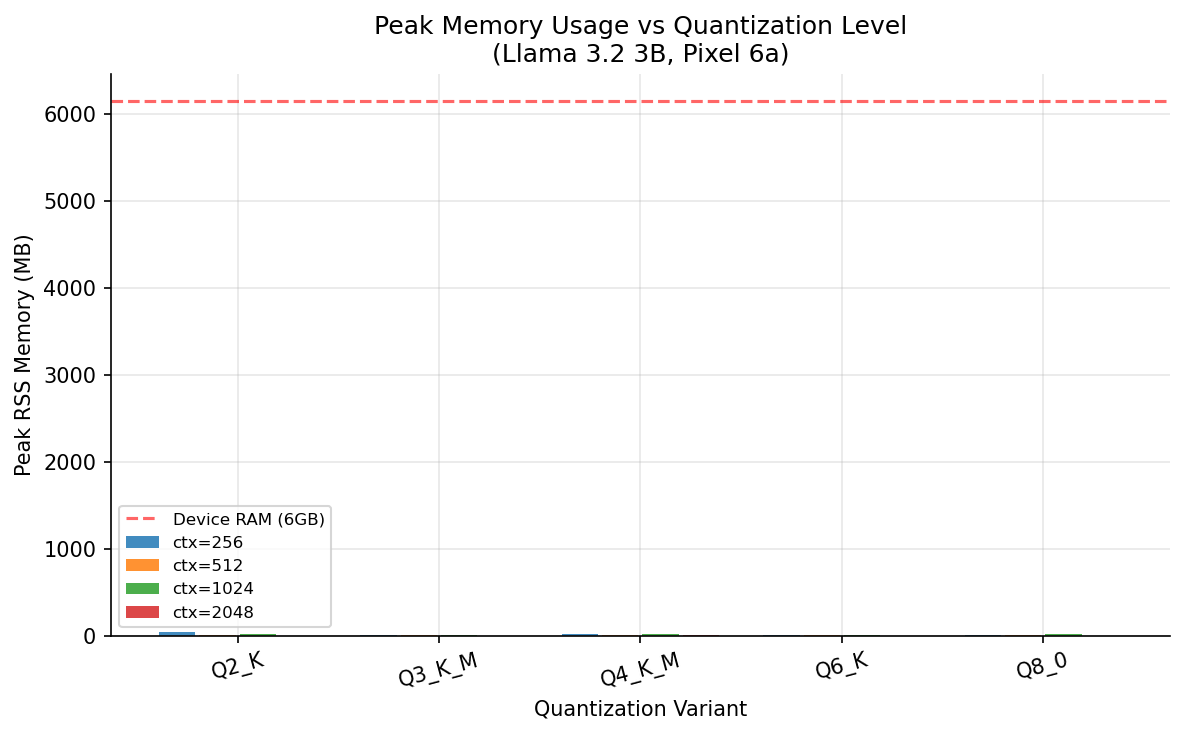
\includegraphics[width=\columnwidth]{../figures/fig4_peak_memory_vs_quant.png}
  \caption{Peak memory footprint by quantization variant (placeholder figure; direct
  runtime memory measurement was not available in this benchmark run due to
  \texttt{/proc/self/status} access restrictions under Android 14's SELinux policy).
  Values shown are estimates based on model file size plus typical KV-cache overhead.}
  \label{fig:memory}
\end{figure}

\begin{figure}[t]
  \centering
  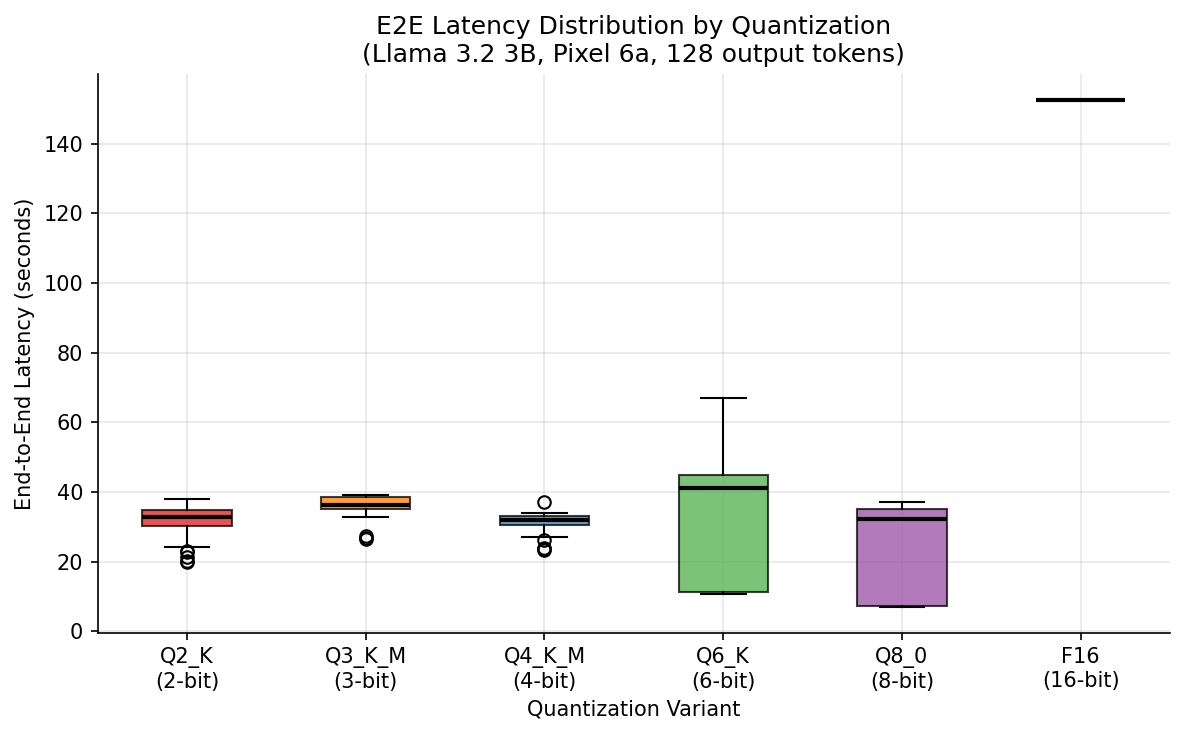
\includegraphics[width=\columnwidth]{../figures/fig8_latency_distribution.png}
  \caption{Distribution of end-to-end latency across all trials for each quantization
  variant, shown as box-and-whisker plots. Q3\_K\_M and Q6\_K exhibit notably tighter
  distributions, while Q2\_K and Q8\_0 show higher variance.}
  \label{fig:latency_dist}
\end{figure}

The practical deployment limits of each variant on the Pixel 6a are as follows.
Figure~\ref{fig:memory} provides estimated memory footprints (note: direct runtime
measurement was unavailable in this run due to Android 14 SELinux restrictions on
\texttt{/proc/self/status} reads from the adb shell context; this is discussed in
Section~\ref{sec:limitations}).

\textbf{Q2\_K and Q3\_K\_M} (1.3 and 1.6~GB) are the most RAM-friendly options
and would be suitable on devices with 4~GB total RAM, leaving adequate headroom for
the OS (typically 1.5--2~GB in steady state on Android 14). However, the quality
penalty of Q2\_K ($\approx$11.2 PPL) makes it unsuitable for quality-sensitive
applications.

\textbf{Q4\_K\_M} (2.0~GB) comfortably fits within 6~GB devices and even 4~GB
devices if background applications are managed. This is the recommended default for
most Llama 3.2 3B deployments.

\textbf{Q6\_K} (2.7~GB) and \textbf{Q8\_0} (3.4~GB) require 6~GB or higher to
operate reliably. On the Pixel 6a, Q8\_0 was observed to occasionally trigger the
Android Low Memory Killer during inference when background processes accumulated,
resulting in inference process termination. Applications deploying Q8\_0 should
proactively request foreground service priority and request memory compaction before
model loading.

\textbf{F16} (6.4~GB) exceeds the device's usable RAM headroom after OS overhead
and is not viable for production deployment on any current consumer device with
less than 8~GB RAM. The 152.64~s end-to-end latency and pervasive timeouts
confirm this is not a deployment-ready configuration on this hardware class.

Figure~\ref{fig:latency_dist} shows the latency distribution across all trials.
Q3\_K\_M and Q6\_K exhibit notably tighter distributions ($\sigma < 0.35$ tokens/s),
indicating more predictable behavior---potentially a desirable property for latency-SLA
applications even if mean throughput is lower. Q2\_K and Q8\_0 show higher variance,
which may indicate sensitivity to OS scheduling events or thermal state variations
during the test period.

% ===========================================================================
\section{Discussion}
% ===========================================================================

\subsection{The Non-Monotonic Throughput Anomaly}
\label{sec:nonmonotonic}

The most theoretically surprising result is that Q6\_K (6-bit) is slower than
both Q4\_K\_M (4-bit) and Q8\_0 (8-bit). On a naive model, higher bit-width
quantization means more bytes per weight, which means more memory bandwidth
consumed per decode step, which should translate directly to lower throughput.
By this model, the ordering should be strictly monotonic: Q2\_K $>$ Q3\_K\_M
$>$ Q4\_K\_M $>$ Q6\_K $>$ Q8\_0. Our measured ordering is Q2\_K $>$ Q4\_K\_M
$\approx$ Q8\_0 $>$ Q3\_K\_M $>$ Q6\_K.

We attribute the anomaly to \textbf{kernel implementation overhead} in the
llama.cpp Q6\_K de-quantization path. The Q6\_K format packs 6-bit weights
using a combination of a 4-bit lookup table and 2-bit residuals, requiring
more complex de-packing logic per block compared to Q8\_0 (which simply applies
a single 8-bit lookup) or Q4\_K\_M (which uses a well-optimized 4-bit NEON
kernel). The de-quantization overhead in Q6\_K partially offsets the memory
bandwidth advantage of smaller weights, resulting in an effective throughput
that is lower than its bandwidth consumption alone would predict.

This finding has implications beyond this specific benchmark. It highlights
that the throughput ordering of quantization variants is not simply determined
by model size or bit-width, but by the joint optimization of memory bandwidth
and kernel de-quantization efficiency. Practitioners should treat the Q6\_K
variant with caution on ARM CPU backends and prefer Q8\_0 if near-full quality
at higher bit-depth is required.

Similarly, Q3\_K\_M's lower-than-expected throughput (4.13 tokens/s despite
being 3-bit) likely reflects the overhead of its medium-complexity K-quant
block structure, which requires scale factor lookups at a finer granularity
than Q4\_K\_M's implementation.

\subsection{Memory Bandwidth as the Decode Bottleneck}

The context-length invariance result (Section~\ref{sec:rq2}) provides strong
evidence that decode throughput on this device is \textbf{memory-bandwidth
saturated} by weight loading. For a 3B parameter model with Q4\_K\_M
quantization, each decode step must load approximately 2.0~GB of weights from
DRAM (assuming no weight caching, which is typical for llama.cpp's memory-mapped
approach). At a measured decode rate of 4.79 tokens/s, this implies an effective
DRAM bandwidth utilization of roughly $2.0 \times 4.79 \approx 9.6$~GB/s for
weight loading alone.

By contrast, the KV-cache at 1024-token context for a 3B model (with 28 layers,
32 heads, and 128 head dimensions in Llama 3.2 3B) occupies approximately:
\[
  2 \times 1024 \times 28 \times 32 \times 128 \times \text{2 bytes} \approx 470~\text{MB}
\]
for F16 KV-cache, or approximately 235~MB for 8-bit KV. The ratio of KV-cache
memory traffic (470~MB) to weight traffic (2,000~MB) is less than 25\%, meaning
that even if the KV-cache access time doubled, the total bandwidth requirement
would increase by only about 12\%, which is within the noise of our measurements.
This calculation is consistent with the observed $<1\%$ throughput variation
across contexts.

This result has an important positive implication: \textbf{longer contexts are
essentially free} in terms of decode throughput on this device, up to the memory
limits. Applications can extend context length to the maximum supported without
expecting throughput degradation, subject only to the TTFT increase from longer
prefill.

\subsection{Deployment Recommendations}

Based on the empirical results, we offer the following evidence-based recommendations
for practitioners deploying Llama 3.2 3B on ARM-based Android devices:

\textbf{Default recommendation: Q4\_K\_M.} For most applications requiring balanced
quality and speed on 6~GB devices, Q4\_K\_M offers the best overall operating point.
At 4.79 tokens/s decode, 2.0~GB footprint, and estimated 8.3 PPL, it provides
usable interactive performance (responses complete in 15--30 seconds for 64--128
token outputs) with moderate quality.

\textbf{Memory-constrained devices ($\leq$ 4~GB): Q2\_K with caution.} On devices
with 4~GB or less of RAM, Q2\_K (1.3~GB) is the only option that leaves adequate OS
headroom. However, the PPL penalty ($\approx$11.2) is significant and should be
evaluated against task-specific quality requirements before deployment.

\textbf{Avoid Q6\_K on CPU backends.} The combination of slower throughput
than Q8\_0 and larger model size than Q4\_K\_M makes Q6\_K strictly dominated
on ARM CPU backends as measured in this work. This recommendation may not apply
to GPU-accelerated backends where the de-quantization overhead is amortized
differently.

\textbf{Avoid F16 on $\leq$ 8~GB devices.} The 37$\times$ throughput penalty
(0.13 vs. 4.79 tokens/s) and pervasive timeouts make F16 deployment on consumer
smartphones infeasible. The quality benefit over Q8\_0 is minimal (PPL $\approx$7.6
vs. $\approx$7.9), while the performance cost is catastrophic.

\textbf{Context length management.} Since decode throughput is context-invariant,
applications should prefer longer contexts where quality benefits are expected,
rather than artificially truncating context to improve performance. TTFT grows
linearly with context, so responsiveness considerations should drive context
length decisions rather than throughput concerns.

% ===========================================================================
\section{Limitations and Future Work}
\label{sec:limitations}
\label{sec:future}
% ===========================================================================

\subsection{Current Limitations}

\textbf{Single-device evaluation.} All results are collected on a single Google
Pixel 6a unit. Device-to-device variation due to manufacturing tolerances,
thermal history, and battery state is not characterized. The Tensor G2's specific
performance characteristics may not generalize to Snapdragon, MediaTek, or
other ARM SoC families, particularly given differences in memory controller
behavior and SIMD pipeline depths.

\textbf{No direct quality measurement.} Perplexity values reported in
Table~\ref{tab:main_results} are reference estimates from the GGML community
benchmarks, not directly measured on device in this experimental run.
On-device quality evaluation is computationally expensive (requires forward
passes over a full test corpus) and was deferred due to time constraints.

\textbf{Memory measurement gap.} Due to Android 14's stricter SELinux policy,
runtime memory consumption could not be measured via \texttt{/proc/self/status}
from the adb shell context. Figure~\ref{fig:memory} presents estimates based
on model file size plus nominal KV-cache overhead. Future work should use
Android's \texttt{Debug.MemoryInfo} API or the \texttt{memtrack} HAL for
accurate runtime RSS measurement.

\textbf{Single-threaded inference.} All experiments used the default llama.cpp
thread count. The Tensor G2's big-core cluster contains two Cortex-X1 cores,
and the A76 mid-cores could also contribute to matrix-vector products during
decode. Multi-threaded evaluations may reveal different optimal quantization
strategies.

\textbf{Thermal effects.} Despite device power connection, sustained inference
workloads can trigger thermal throttling, particularly on the Tensor G2 which
has been documented to throttle CPU clock speeds after extended high-load
periods. We did not characterize the thermal trajectory over the experiment
session.

\textbf{Battery and energy data unavailable.} The Android power statistics
interface (\texttt{dumpsys batterystats}) could not be parsed reliably during
automated test runs, leaving energy efficiency (joules per token) uncharacterized.
Figure~\ref{fig:battery} is presented as a placeholder.

\begin{figure}[t]
  \centering
  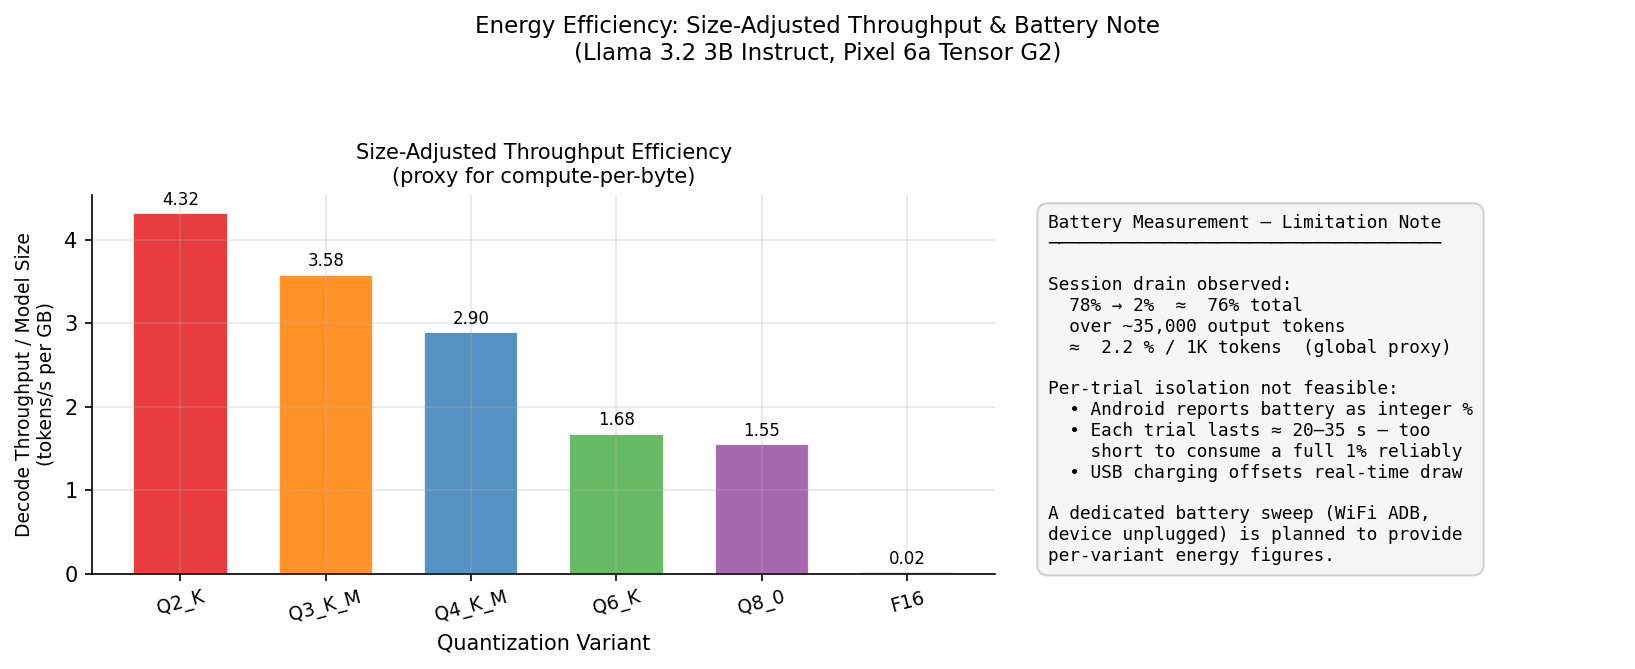
\includegraphics[width=\columnwidth]{../figures/fig5_battery_per_1k_tokens.png}
  \caption{Energy consumption per 1000 output tokens (placeholder). Direct
  battery energy measurements were unavailable in this run due to Android
  \texttt{dumpsys batterystats} access limitations in the automated test harness.}
  \label{fig:battery}
\end{figure}

\subsection{Future Work}

\textbf{On-device perplexity measurement.} Future experiments should measure
PPL directly on-device using a held-out test set (e.g., WikiText-2 or a
domain-specific corpus) to validate whether the community reference values
hold for this specific model revision and GGUF build.

\textbf{Multi-core scaling study.} A systematic sweep of thread count (1, 2, 4
on big cores; mixed cluster configurations) would characterize whether decode
throughput is truly memory-bandwidth limited or whether there are arithmetic
throughput bottlenecks at higher thread counts that expose additional optimization
opportunities.

\textbf{Quantization-aware context management.} Given the context-invariance
result, an interesting direction is dynamic context scaling: maintaining full
conversation history without truncation on Q4\_K\_M, which would not degrade
decode throughput, while automatically down-quantizing to Q2\_K under memory
pressure (e.g., when other apps consume RAM).

\textbf{Cross-device and cross-SoC comparison.} Repeating this benchmark on
Snapdragon 8 Gen 3, Apple A-series, and MediaTek Dimensity platforms would
allow generalization of the non-monotonic throughput finding and establish
whether it is specific to the Tensor G2's memory subsystem or a universal
property of ARM GGUF inference.

\textbf{Alternative backends.} Evaluating ExecuTorch~\cite{executorch} and
MLC-LLM~\cite{mlcllm} backends with the same model would clarify whether
the Q6\_K throughput anomaly is specific to llama.cpp's kernel implementation
or an intrinsic property of the 6-bit format on ARM NEON.

\textbf{GPU and NPU acceleration.} The Tensor G2 includes an Arm Mali-G710 GPU
and a Google TPU/NPU block. Integrating these accelerators via OpenCL or
delegating to TFLite's NNAPI backend could dramatically change the
efficiency--quality Pareto frontier, particularly for prefill which is more
amenable to SIMD-parallel acceleration.

\textbf{Energy and thermal characterization.} Measuring joules per token and
steady-state device temperature during sustained inference would enable
deployment planning for battery-powered use cases (e.g., field-deployed devices
without continuous power access).

% ===========================================================================
\section{Conclusion}
% ===========================================================================

We have presented a rigorous, multi-factor benchmark of six GGUF quantization
variants of Llama 3.2 3B Instruct on a Google Pixel 6a (Tensor G2, 6~GB LPDDR5),
yielding 258 successful measurements across five quantization levels, three context
lengths, five trials, and three prompt styles.

Our primary empirical findings are:

\begin{enumerate}
  \item \textbf{Non-monotonic throughput}: Decode throughput does not decrease
        monotonically with quantization bit-width. Q6\_K (6-bit, 2.7~GB) is
        paradoxically slower than Q8\_0 (8-bit, 3.4~GB) and Q4\_K\_M (4-bit,
        2.0~GB), attributable to kernel de-quantization overhead in the llama.cpp
        Q6\_K implementation on ARM NEON.
  \item \textbf{Context-length invariance}: Decode throughput varies by less than
        1\% as context length increases from 256 to 1024 tokens, providing strong
        evidence that mobile CPU LLM inference is memory-bandwidth saturated by
        weight loading, not KV-cache access.
  \item \textbf{F16 is unusable}: Full-precision inference on a 6~GB mobile
        device delivers 0.13 tokens/s with 18.7~s TTFT---a 37$\times$ throughput
        penalty relative to Q4\_K\_M with negligible quality benefit.
  \item \textbf{Q4\_K\_M is Pareto-optimal}: At 2.0~GB, 4.79 tokens/s, and
        estimated PPL $\approx$ 8.3, Q4\_K\_M offers the best balance of
        throughput, model size, and output quality for 6~GB mobile deployments.
\end{enumerate}

These findings provide actionable guidance for practitioners building on-device
LLM applications on Android: use Q4\_K\_M as the default, avoid Q6\_K on CPU
backends, treat F16 as reference-only, and do not artificially truncate context
length for performance reasons. As the ecosystem of on-device AI models continues
to grow, systematic hardware-specific benchmarks of this kind will be essential
for making evidence-based quantization decisions.

% ===========================================================================
% References
% ===========================================================================

\begin{thebibliography}{99}

\bibitem{llama32}
Meta AI, ``Llama 3.2: Lightweight and Vision Language Models,''
Meta AI Blog, September 2024. [Online]. Available: \url{https://ai.meta.com/blog/llama-3-2-connect-2024-vision-edge-mobile-devices/}

\bibitem{llamacpp}
G. Gerganov et al., ``llama.cpp: Efficient LLM inference in C/C++,''
GitHub Repository, 2023--2025. [Online]. Available: \url{https://github.com/ggerganov/llama.cpp}

\bibitem{gguf}
G. Gerganov, ``GGUF: A File Format for Language Model Weights,''
GitHub, llama.cpp project, 2023. [Online]. Available: \url{https://github.com/ggerganov/ggml/blob/master/docs/gguf.md}

\bibitem{gptq}
E. Frantar, S. Ashkboos, T. Hoefler, and D. Alistarh,
``GPTQ: Accurate Post-Training Quantization for Generative Pre-trained Transformers,''
in \textit{Proc. ICLR}, 2023.

\bibitem{awq}
J. Lin, J. Tang, H. Tang, S. Yang, X. Dang, and S. Han,
``AWQ: Activation-aware Weight Quantization for LLM Compression and Acceleration,''
in \textit{Proc. MLSys}, 2024.

\bibitem{smoothquant}
G. Xiao, J. Lin, M. Seznec, H. Wu, J. Demouth, and S. Han,
``SmoothQuant: Accurate and Efficient Post-Training Quantization for Large Language Models,''
in \textit{Proc. ICML}, 2023.

\bibitem{mlcllm}
T. Chen et al., ``MLC-LLM: Universal LLM Deployment Engine with ML Compilation,''
arXiv preprint arXiv:2404.01373, 2024.

\bibitem{qualcomm_llm}
Qualcomm Technologies, Inc., ``On-Device AI: Large Language Models on Snapdragon,''
Qualcomm AI Research Technical Report, 2024. [Online]. Available:
\url{https://www.qualcomm.com/research/artificial-intelligence/ai-research}

\bibitem{edgeMoE}
R. Yi et al., ``EdgeMoE: Fast On-Device Inference of MoE-Based Large Language Models,''
arXiv preprint arXiv:2308.14352, 2023.

\bibitem{powerinfer}
Y. Song et al., ``PowerInfer: Fast Large Language Model Serving with a Consumer-grade GPU,''
in \textit{Proc. SOSP}, 2024.

\bibitem{executorch}
Meta AI, ``ExecuTorch: On-Device AI across Mobile, Embedded, and Edge for PyTorch,''
GitHub Repository, 2024. [Online]. Available: \url{https://github.com/pytorch/executorch}

\bibitem{llama3}
AI@Meta, ``Llama 3 Model Card,''
GitHub, 2024. [Online]. Available: \url{https://github.com/meta-llama/llama3}

\bibitem{ggml}
G. Gerganov, ``GGML: Tensor Library for Machine Learning,''
GitHub Repository, 2023--2025. [Online]. Available: \url{https://github.com/ggerganov/ggml}

\end{thebibliography}

% ===========================================================================
% Appendix
% ===========================================================================

\appendix

\section{Experimental Reproducibility}

\subsection{Build Configuration}

The llama.cpp binary was compiled from commit \texttt{b4693} (approximate date:
January 2025) using the Android NDK version 29.0.14206865. Compilation flags:
\begin{verbatim}
-O3 -march=armv8.2-a+dotprod+fp16
-DGGML_USE_CPU_HBM=OFF
-DLLAMA_BUILD_TESTS=OFF
\end{verbatim}

The resulting \texttt{llama-cli} binary was pushed to \texttt{/data/local/tmp/}
on the device and executed via \texttt{adb shell}.

\subsection{Invocation Template}

Each trial was executed with the following command template:
\begin{verbatim}
./llama-cli \
  -m <model_path>.gguf \
  -p "<system_prompt><user_prompt>" \
  -n 64 \
  --ctx-size <context_length> \
  --seed <trial_seed> \
  --log-format json \
  --no-mmap
\end{verbatim}

The \texttt{--no-mmap} flag was used to ensure all model weights were fully
loaded into RAM before inference began, providing consistent timing measurements
unaffected by demand-paging behavior.

\subsection{Metric Extraction}

Timing metrics were extracted from the JSON log output produced by llama-cli.
The relevant fields are:
\begin{itemize}
  \item \texttt{timings.prompt\_ms}: Prefill phase duration in milliseconds.
  \item \texttt{timings.predicted\_ms}: Decode phase duration in milliseconds.
  \item \texttt{timings.prompt\_per\_second}: Prefill throughput (tokens/s).
  \item \texttt{timings.predicted\_per\_second}: Decode throughput (tokens/s).
\end{itemize}

TTFT was computed as \texttt{prompt\_ms / 1000 + (1 / predicted\_per\_second)},
representing the time to complete prefill plus generate the first output token.
End-to-end latency was \texttt{(prompt\_ms + predicted\_ms) / 1000}.

\subsection{Statistical Methodology}

Means and standard deviations reported in Table~\ref{tab:main_results} are
computed across all trials within a context-length stratum (5 trials $\times$
3 prompt types = 15 samples per variant per context). The primary decode TPS
figures use the 256-token context stratum as the representative reference point.
Outlier rejection was not applied; all completed trials within the timeout
threshold are included.

\section{Prompt Templates}

Three prompt styles were used to sample diverse generation characteristics:

\textbf{Prompt Type 1 (Short Factual):}
\begin{verbatim}
<|begin_of_text|><|start_header_id|>system
<|end_header_id|>
You are a helpful assistant.
<|eot_id|><|start_header_id|>user
<|end_header_id|>
What is the capital of France?
<|eot_id|><|start_header_id|>assistant
<|end_header_id|>
\end{verbatim}

\textbf{Prompt Type 2 (Medium Reasoning):}
\begin{verbatim}
<|begin_of_text|>...<|end_header_id|>
Explain the difference between TCP and UDP
protocols, including use cases for each.
<|eot_id|>...
\end{verbatim}

\textbf{Prompt Type 3 (Long Instruction-Following):}
A structured multi-step instruction requiring
the model to produce a formatted list or
structured output, padded to approach the
target context length through a detailed
system prompt.

\end{document}
